\documentclass[a4paper,11pt,twoside]{article}
%\documentclass[a4paper,11pt,twoside,se]{article}

\usepackage{UmUStudentReport}
\usepackage{verbatim}   % Multi-line comments using \begin{comment}
\usepackage{courier}    % Nicer fonts are used. (not necessary)
\usepackage{pslatex}    % Also nicer fonts. (not necessary)
\usepackage[pdftex]{graphicx}   % allows including pdf figures
\usepackage{listings}
\usepackage{pgf-umlcd}
\usepackage{blindtext}
\usepackage{enumitem}
\usepackage{amsmath}
\usepackage{amssymb}
%\usepackage{lmodern}   % Optional fonts. (not necessary)
%\usepackage{tabularx}
%\usepackage{microtype} % Provides some typographic improvements over default settings
%\usepackage{placeins}  % For aligning images with \FloatBarrier
%\usepackage{booktabs}  % For nice-looking tables
%\usepackage{titlesec}  % More granular control of sections.

% DOCUMENT INFO
% =============
\department{Department of Computing Science}
\coursename{Parallel Programming 7.5 p}
\coursecode{5DV152}
\title{Exercises, Chapter/Topic 6}
\author{Lorenz Gerber ({\tt{dv15lgr@cs.umu.se}} {\tt{lozger03@student.umu.se}})}
\date{2017-03-09}
%\revisiondate{2016-01-18}
\instructor{Lars Karlsson / Mikael Ränner}


% DOCUMENT SETTINGS
% =================
\bibliographystyle{plain}
%\bibliographystyle{ieee}
\pagestyle{fancy}
\raggedbottom
\setcounter{secnumdepth}{2}
\setcounter{tocdepth}{2}
%\graphicspath{{images/}}   %Path for images

\usepackage{float}
\floatstyle{ruled}
\newfloat{listing}{thp}{lop}
\floatname{listing}{Listing}



% DEFINES
% =======
%\newcommand{\mycommand}{<latex code>}

% DOCUMENT
% ========
\begin{document}
\lstset{language=C}
\maketitle
\thispagestyle{empty}
\newpage
\tableofcontents
\thispagestyle{empty}
\newpage

\clearpage
\pagenumbering{arabic}

\section{Introduction}
This report is part of the mandatory coursework. It describes the solutions for several chosen exercises from the course book \cite{pacheco2011}.

\section{Modification of $n$ body solver}
Yes it would be possible to remove the the inner \verb+for+ loop. However, as the calculation of force makes use of the position of all particles, updates to the position would need to be stored in a temporary variable and updated after calculating the force for all particles of the current step. This would probably deteriorate a potential speed gain from removing some structure again.

\section{Extrapolation of execution time for $n$ body solver}
The serial n-body solver was run according to the specifications in the book for 500 to 2000 particles with 3 replicates. The timings were then plotted as shown in figure \ref{fig:nbody.png}. From the plot shape, a transformation was guessed ($x^2$). Then a linear model was fitted and extrapolated to 24h. The approximation for 24h was 70'000 particles.

\begin{figure}
  \centering
  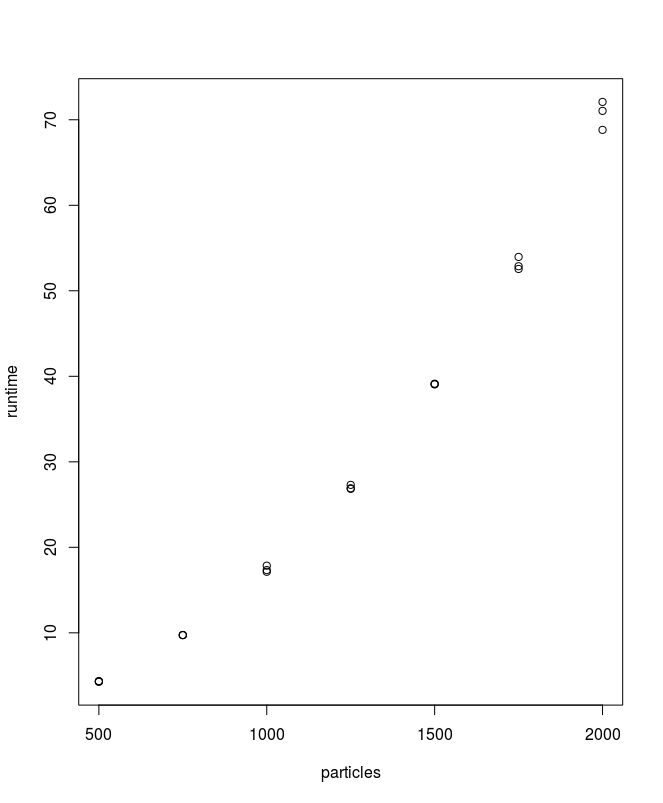
\includegraphics[width=1\textwidth]{nbody.png}
  \caption{\textit{This figure shows the measured timings from running the nbody solver with 1000 time steps of step size 0.75 in range for particles from 500 to 2000. The graph was used to estimate a good transformation function. Here $x^2$ was found to be suitable }}
  \label{fig:nbody}
\end{figure}

\section{Eliminating implied barriers}
Eliminating the implied barriers in the basic OpenMP implementation has a similar consequence as described in question 6.1. As calculation of the force on particles needs the position information of each and every particle, threads that `run' ahead to the position update block and change the positions while others still calculate the force would result in wrong force values and as a consequence also false positions. Hence, removing the implied barriers would result in a wrong and unpredictable result.
  
\section{DAXPY}
Here a \textit{DAXPY} calculation was implemented using OpenMP. The source code can be seen below. The aim was to test the influence of using either a block or a cyclic partitioning for the scheduling of the parallel for loops. While cyclic partitioning is obtained by using the \verb+schedule(static, 1)+ clause. For block partitioning $array_length \div cores$ was used as value $n$ in the \verb+schedule(static, n)+ clause.

 The result in terms of run times using an increasing number of cores can be seen in figure \ref{fig:daxpy}. It is obvious that the block partitioning performs better and more consistent for all instances of core numbers. While block partitioning is always faster, it's run times are generally also subjected to less variation compared to cyclic partitioning.

The reason for the difference in performance should be the memory access. It is much more efficient when a thread can access and use non-interrupted ranges of memory addresses as it is the case with block partitioning.  
 
\begin{verbatim}
#include <stdio.h>
#include <stdlib.h>
#include "timer.h"
#include <omp.h>
#include <string.h>


int main(int argc, char *argv[]){

  double a;
  double* x;
  double* y;
  int i;
  int thread_count = strtol(argv[1], NULL, 10);
  int n = strtol(argv[2], NULL, 10);
  int c = strtol(argv[3], NULL, 10);
  
  double start, finish;

  x = malloc(n * sizeof(double));
  y = malloc(n * sizeof(double));
  
  srand(0);
  a = rand();
  for (i = 0; i < n; i++){
    x[i] = rand();
    y[i] = rand();
  }
  
  GET_TIME(start);

# pragma omp parallel private(i) num_threads(thread_count)
  {

#   pragma omp for schedule(static, c)
    for (i = 0; i < n; i++)
      x[i]=a*x[i];
#   pragma omp for schedule(static, c)
    for(i = 0; i < n; i++)
      y[i] = x[i] + y[i];
  }

  GET_TIME(finish);

  printf("%d %d %e\n", thread_count, c, (finish-start));

  free(x);
  free(y);

  return 0;
}

\end{verbatim}

\begin{figure}
  \centering
  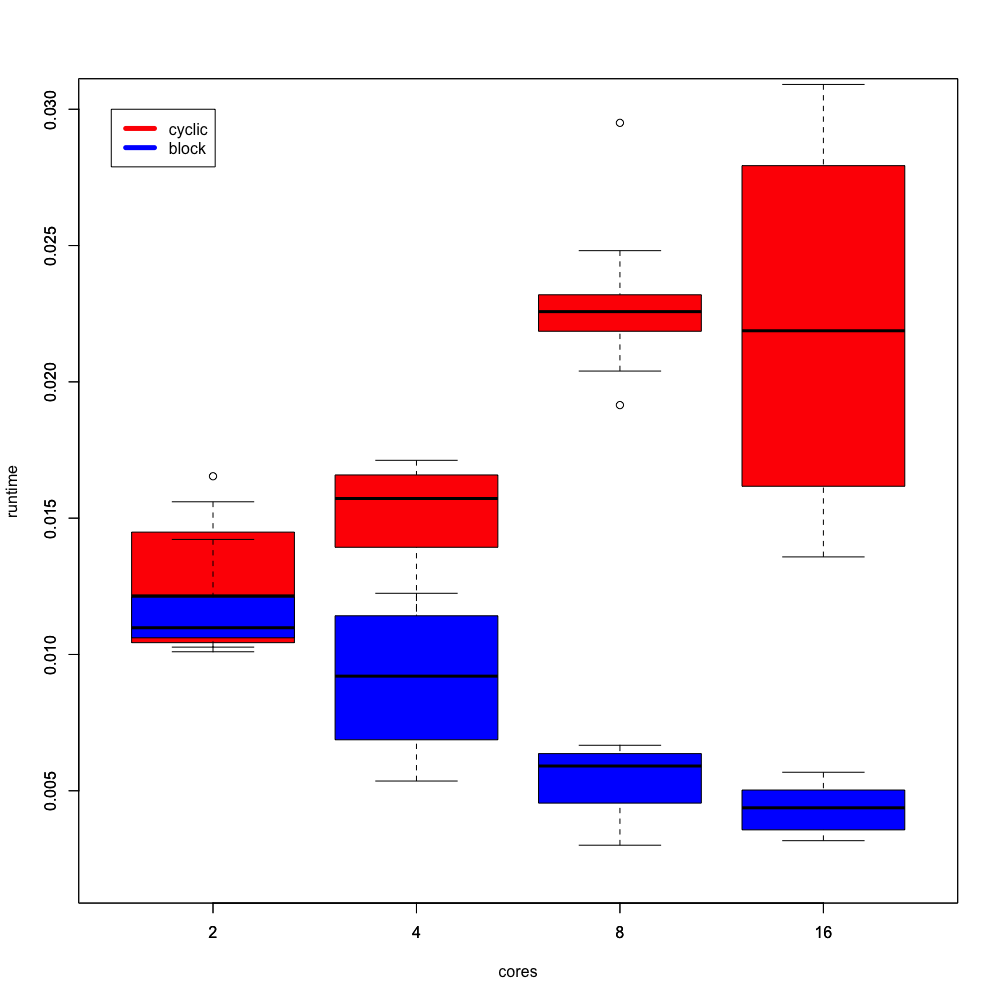
\includegraphics[width=1\textwidth]{daxpy.png}
  \caption{\textit{This figure shows the measured timings from running the omp\_daxpy.c program with either cyclic or block partitioning on 1'000'000 n arrays using $\{2, 4, 8, 16\}$ cores on the HPC2N `abisko' cluster. It is obvious that a pure cyclic scheduling is sub-optimal as here threads can not work on uninterrupted ranges of memory which significantly slows down the calculation.}}
  \label{fig:daxpy}
\end{figure}

\section{L2 cache misses}
The aim here was to analyze a program consisting of two loops and determine for the second loop the number of cache misses under two different chunk-sizes, \verb+n/thread_count+ and \verb+8+. It is important to notice that the chunk-size in the first \verb+for+ loop is \verb+n/thread_count+. In the \verb+schedule+ clause of OpenMP, this can be interpreted as block partitioning. In the current setup a cache-line holds 8 doubles and the number of doubles in the two arrays of interest are 64. Hence, in the first \verb+for+ loop each core, which by definition has it's own L2 cache, will have access to each 32 doubles in 4 cache lines (4 cache lines at each core). Using block partitioning in the first \verb+for+ loop should yield doubles of the arrays $x$ and $y$ with indices $\{0...31\}$ to end up in the L2 cache of core $0$ and those with indices $\{32...63\}$ at core $1$.

\subsection*{chunksize = n/thread\_count}
When now the schedule clause in the second \verb+for+ loop is identical to the first, it can be assumed that each core will get the indices of the loop to which there are the corresponding array entries in the L2 cache. Hence this setup results in zero cache misses.
 
\subsection*{chunksize = 8}
Here for the second \verb+for+ loop, block partitioning with chunk-size 8 was chosen. As one cache line holds 8 doubles, from the total of 8 cache lines assigned during the first loop (8 per array, hence 16 for both $x$ and $y$), 4 are in the L2 of the `wrong' core. Hence, 4 cache misses per array (8 for both $x$ and $y$) will result. 

Another detail is that in this configuration, 32 doubles on 4 cache lines happen to be in the cache of the `wrong' core for the second loop. However, when a cache miss happens, a whole cache line is read again, therefore the following 7 doubles will no longer result in cache misses.  

\section{Local/global index conversions}
To devise formulas for translation from global to local indices and vice versa, the following variables are used: $k$ for rank, $b$ for block-size, $l$ for local index and $g$ for global index.

\begin{enumerate}[label={\alph*)}]
\item global index from local for block distribution
\begin{equation*}
k \times b + l
\end{equation*}
\item local from global for block distribution
\begin{equation*}
g \mod b
\end{equation*}
\item global from local for cyclic distribution
\begin{equation*}
(g-k) \div b
\end{equation*}
\item local from global for cyclic distribution
\begin{equation*}
l \times b + k
\end{equation*}
\end{enumerate}


\section{Stack splitting in TSP}
In the dynamic TSP code, several different stack splitting strategies are first discussed theoretically, then they were implemented and evaluated by a benchmark runs.
\begin{enumerate}[label={\alph*)}]
\item Splitting the stack half, $k/2$\\
The stack is in general built up by adding new partial tours with increasing number of cities. Hence splitting the stack in half will result with the old stack containing just short partial tours with potentially still a lot of work left, while the new stack gets all the long partial tours that are potentially soon determined. Obviously, this is not a very even load balancing.
\item Sorting for tour length, divide round robin\\
Here the stack is first sorted according to the total cost of partial tours and then round-robin distributed between the old and the new stack. This should definitively be an improvement over the prior $k/2$ division. But comparing the cost between very short and very long partial tours misses another important factor to equally distribute the work. It can still happen that one stack ends up with mostly short partial tours that still demand a lot of work or vice versa with mostly tours that are almost finished.
\item Sorting for tour-length-divided-by-number-of-edges, divide round robin\\
Sorting the partial tours first for total cost divided by number of edges to obtain some sort of average cost can be seen as a synthesis of the prior mentioned strategy and the one implemented in pth\_tsp\_dyn. Same as in the prior method, after sorting the partial tours are distributed in a round-robin fashion between the old and the new stack. This method should potentially perform better than the other strategies so far. 
\end{enumerate}

All programs were implemented using the pthread `dynamic tsp' program as basis. Beside sort comparator functions, all code to be changed was within the \verb+Split_stack+ function. The source code for the \textit{k/2} implementation can be found in appendix \ref{app:k2}, for the \textit{least-cost} implementation in appendix \ref{app:cost} and for the \textit{average cost per edge} in appendix \ref{app:avgcost}.  

The implemented programs were run batch run for benchmarking on the HPC2N cluster. Each measurement was repeated five times. Looking at individual boxplots (not shown) it was obvious that variation within replicates was small, hence the data was summarized using median values in table \ref{tab:tsp}.

\begin{table}[]
\centering
\caption{\textit{This table shows run times in seconds from comparing various version of the Traveling Salesman Problem algorithm. The difference between the various versions is how the stack is split when one thread runs out of work. Timings were collected on the HPC2N `Abisko' cluster. The data matrix with the travel costs was of the size n = 13.}}
\label{tab:tsp}
\begin{tabular}{l|cccc}
cores & dynamic & k/2   & cost  & avg cost \\ \hline
1     & 78.09   & 77.50 & 78.40 & 77.43    \\
2     & 41.13   & 41.53 & 40.79 & 40.42    \\
4     & 22.29   & 22.14 & 22.26 & 22.17    \\
8     & 12.85   & 12.95 & 12.97 & 12.67   
\end{tabular}
\end{table}

The results of the benchmarking suggest that the strategy of stack splitting had no large influence on the run times. However, as variation in run-times was small, it is anyhow possible to see tendencies in the performance of the different strategies. The simplest method \textit{k/2} performed consistently worse than any other implementation (expect for the 1 core case. Here the behavior would have to be investigated more but it seems not really relevant for the evaluation of the actual stack splitting strategies which is the topic here). The parallel performance of the \textit{k/2} strategy was also mostly worse than all the others. For some reason that would need to be investigated more, the \textit{k/2} strategy performed however best running on four cores.

Else it can be seen that both the \textit{minimal cost} and the \textit{minimal average cost} strategy usually outperform the given implementation that sorts according to tour length before splitting. As it was assumed, the \textit{minimal average cost} strategy performed slightly better than the \textit{minimal cost} strategy.

The current data was recorded using a $n = 13$ matrix and a stack split cut-off value of 10. While writing this text, another batch run is attempted to check whether a lower stack-split cut-off would have a significant influence on the various methods (without having evaluated the run with cut-off 4 numerically, it was obvious from looking through the run-times that they were not much changed).  

\section{Choosing an API}
\subsection{Memory Requirement}
\subsubsection{nbody solvers}
\begin{enumerate}
\item The memory requirement for the serial nbody solver slightly lower than for the reduced one as it uses two additional arrays (\verb+force_qk+).
\item The parallel version of shared memory implementations will use significantly more memory for the reduced  nbody solver as there need to be made local copies of the force table for each thread. Hence memory usage increases linear with number of threads. To compare the memory usage between shared memory and distributed memory implementation of the nbody solver, the amount of local memory in the distributed system is compared to the amount of memory needed in the shared memory system. 
In the basic version, the MPI implementation needs some more local storage than the shared memory version. In the reduced version, however, for large numbers of particles, the amount of local memory required for the MPI implementation is significantly lower than for the shared memory implementation.
\end{enumerate}
\subsubsection{TSP}
For the TSP program, memory usage is generally not much of a problem, neither in the serial nor in the parallel implementation, independent of static or dynamic task mapping.  
\subsection{Communication Requirement}
\subsubsection{nbody solver}
The communication requirements for the nbody solver are generally low. For the shared memory systems, it is limited to synchronization between different for loops, both in the basic and in the reduced version. For the shared memory system, however, a lot of communication takes place as matrices need to be updated across the various nodes. The communication in the basic version uses rather standard communication protocols such as Allgather etc. The amount of communication can be varied as a compromise between memory usage and amount of communication as certain variables don't change during the whole calculation, so they can either be stored on each node (high memory usage) or requested when used (increased communication). For the reduced distributed-memory implementation of the nbody solver, some special communication concepts need to be applied to make it feasible with a reasonable amount of communication. The course book demonstrates the use of ring-pass communication. 

\subsubsection{TSP}
Communication for the shared-memory implementation of TSP with static mapping is rather low. Initially, each thread will get it's start tasks assigned, then threads can in principle work autonomously until termination. The current implementation included however a communication step to update the best-tour found so far. This can lead to run-time optimization when a thread realizes that his current part tour is already over the current best. Obviously more communication steps are needed if the workload shall be shared dynamically during run time. Here, the difference between shared-memory and distributed-memory is not large. An additional communication step, that needs to be implemented in all systems is the termination detection. 

\subsection{Ease of Parallelization by OpenMP directives}
\subsubsection{nbody solver}
Both the basic and reduced nbody are straight forward to implement on OpenMP. Here, a large advantage of OpenMP is the built in scheduling possibility.
\subsubsection{TSP}
The TSP algorithm uses a lot more communication which probably can be said is not the strongest side of OpenMP. Therefore, pthread felt more suited as it allows a more fine-grained control of processes and communication among threads. For example, it was needed to use busy waiting in the OpenMP implementation as replacement for conditional variables in pthread.

\addcontentsline{toc}{section}{\refname}
\bibliography{references}

\appendix
\section{C Source Code TSP \textit{k/2}}{\label{app:k2}}
\begin{verbatim}
/*------------------------------------------------------------------
 * Function:  Split_stack
 * Purpose:   Return a pointer to a new stack, nonempty stack
 *            created by dividing the orginal stack into two parts.
 * In/out arg:  stack
 * Ret val:     new stack
 */
my_stack_t Split_stack(my_stack_t stack, long my_rank) {
  int new_src, new_dest;//, old_src, old_dest;
   my_stack_t new_stack = Init_stack();

#  ifdef TERM_DEBUG
   Print_stack(stack, my_rank, "Original old stack");
#  endif

   new_dest = 0;
   for (new_src = stack->list_sz/2; new_src < stack->list_sz; new_src++) {
      new_stack->list[new_dest++] = stack->list[new_src];
   }

   new_stack->list_sz = stack->list_sz/2 + stack->list_sz%2;
   stack->list_sz = stack->list_sz/2;
   

#  ifdef TERM_DEBUG
   Print_stack(stack, my_rank, "Updated old stack");
   Print_stack(new_stack, my_rank, "New stack");
#  endif

   return new_stack;
}  /* Split_stack */
\end{verbatim}

\section{C Source Code TSP \textit{cost}}{\label{app:cost}}
\begin{verbatim}
/*------------------------------------------------------------------
 * Function:  Split_stack
 * Purpose:   Return a pointer to a new stack, nonempty stack
 *            created by taking half the records on the input stack
 *            sorted ascending according part tour cost
 * In/out arg:  stack
 * Ret val:     new stack
 */
my_stack_t Split_stack(my_stack_t stack, long my_rank) {
   int new_src, new_dest, old_src, old_dest;
   
   my_stack_t new_stack = Init_stack();
   
#  ifdef TERM_DEBUG
   Print_stack(stack, my_rank, "Original old stack");
#  endif

   qsort((void*)stack->list, stack->list_sz, sizeof(tour_t), comp_cost);

   new_dest = 0;
   old_dest = 1;
   for (new_src = 1; new_src < stack->list_sz; new_src += 2) {
      old_src = new_src+1;
      new_stack->list[new_dest++] = stack->list[new_src];
      if (old_src < stack->list_sz) 
         stack->list[old_dest++] = stack->list[old_src];
   }

   stack->list_sz = old_dest;
   new_stack->list_sz = new_dest;

#  ifdef TERM_DEBUG
   Print_stack(stack, my_rank, "Updated old stack");
   Print_stack(new_stack, my_rank, "New stack");
#  endif

   return new_stack;
}  /* Split_stack */


/*------------------------------------------------------------------           
 * Function:  comp_cost
 * Purpose:   comperator used in Split_stack
 * Out global:  int value interpreted by qsort for ascending 
 * of part tour cost 
 */
int comp_cost(const void *v1, const void *v2) {
  int result;
  tour_t p1 = (tour_t)v1;
  tour_t p2 = (tour_t)v2;
  result = p1->cost - p2->cost;
  return result;
}

\end{verbatim}

\section{C Source Code TSP \textit{average cost per edge}}{\label{app:avg_cost}}

\begin{verbatim}
/*------------------------------------------------------------------
 * Function:  Split_stack
 * Purpose:   Return a pointer to a new stack, nonempty stack
 *            created by taking half the records on the input stack
 *            ordered according ascending average cost per edge
 * In/out arg:  stack
 * Ret val:     new stack
 */
my_stack_t Split_stack(my_stack_t stack, long my_rank) {
   int new_src, new_dest, old_src, old_dest;
   
   my_stack_t new_stack = Init_stack();
   
#  ifdef TERM_DEBUG
   Print_stack(stack, my_rank, "Original old stack");
#  endif

   qsort((void*)stack->list, stack->list_sz, sizeof(tour_t), comp_avg_cost);

   new_dest = 0;
   old_dest = 1;
   for (new_src = 1; new_src < stack->list_sz; new_src += 2) {
      old_src = new_src+1;
      new_stack->list[new_dest++] = stack->list[new_src];
      if (old_src < stack->list_sz) 
         stack->list[old_dest++] = stack->list[old_src];
   }

   stack->list_sz = old_dest;
   new_stack->list_sz = new_dest;

#  ifdef TERM_DEBUG
   Print_stack(stack, my_rank, "Updated old stack");
   Print_stack(new_stack, my_rank, "New stack");
#  endif

   return new_stack;
}  /* Split_stack */


/*------------------------------------------------------------------           
 * Function:  comp_cost
 * Purpose:   comperator used in Split_stack
 * Out global:  int value interpreted by qsort for ascending
 * average cost per edge
 */
int comp_avg_cost(const void *v1, const void *v2) {
  double result;
  tour_t p1 = (tour_t)v1;
  tour_t p2 = (tour_t)v2;
  result = (double)p1->cost/(double)p1->count - (double)p2->cost/(double)p2->count;
  if (result < 0)
    return -1;
  else if (result > 0)
    return 1;
  else
    return 0;
}
\end{verbatim}

\end{document}
